 % !TEX program  = xelatex
% !TEX encoding = UTF-8 Unicode
%
% 编译命令（执行两次生成完整目录与引用）：
%   xelatex 小题大Drama_说明文档.tex
%   xelatex 小题大Drama_说明文档.tex
%
% 依赖：TeX Live 2022+ 或 MiKTeX 22+（含 ctex、tikz、geometry、
%        booktabs、enumitem、titlesec、fancyhdr、hyperref、tcolorbox）

\documentclass[10pt, a4paper]{article}

%%═══════════════════════════════════════════════════════════════
%% 中文支持（XeLaTeX + ctex）
%%═══════════════════════════════════════════════════════════════
\usepackage[UTF8, heading=true]{ctex}

%%═══════════════════════════════════════════════════════════════
%% 页面布局（缩小页边距，10pt 基准，提升信息密度）
%%═══════════════════════════════════════════════════════════════
\usepackage{geometry}
\geometry{
  a4paper,
  top      = 1.8cm,
  bottom   = 1.8cm,
  left     = 2.0cm,
  right    = 2.0cm,
  headheight = 14pt
}

%%═══════════════════════════════════════════════════════════════
%% 排版工具包
%%═══════════════════════════════════════════════════════════════
\usepackage{setspace}
\usepackage{float}
\usepackage{enumitem}
\usepackage{booktabs}
\usepackage{array}
\usepackage{tabularx}
\usepackage{multirow}
\usepackage{xcolor}
\usepackage{titlesec}
\usepackage{fancyhdr}
\usepackage{graphicx}
\usepackage{caption}
\usepackage{hyperref}

%%═══════════════════════════════════════════════════════════════
%% tcolorbox（高亮框，个性化排版）
%%═══════════════════════════════════════════════════════════════
\usepackage[skins]{tcolorbox}

%%═══════════════════════════════════════════════════════════════
%% TikZ
%%═══════════════════════════════════════════════════════════════
\usepackage{tikz}
\usetikzlibrary{
  shapes.geometric,
  arrows.meta,
  positioning,
  fit,
  backgrounds,
  calc
}

%%═══════════════════════════════════════════════════════════════
%% 颜色定义
%%═══════════════════════════════════════════════════════════════
\definecolor{AppleBlue}{RGB}{0,122,255}
\definecolor{LightBlue}{RGB}{218,234,255}
\definecolor{DarkGray}{RGB}{44,44,46}
\definecolor{MidGray}{RGB}{110,110,118}
\definecolor{LightGray}{RGB}{242,242,247}
\definecolor{TokenPurple}{RGB}{88,68,200}
\definecolor{SoftPurple}{RGB}{234,230,255}
\definecolor{SupaGreen}{RGB}{45,170,100}
\definecolor{SoftGreen}{RGB}{212,244,228}
\definecolor{WarnOrange}{RGB}{215,105,0}
\definecolor{SoftOrange}{RGB}{255,242,212}
\definecolor{RuleGray}{RGB}{210,210,218}

%%═══════════════════════════════════════════════════════════════
%% hyperref 配置
%%═══════════════════════════════════════════════════════════════
\hypersetup{
  colorlinks = true,
  linkcolor  = DarkGray,
  urlcolor   = AppleBlue,
  citecolor  = AppleBlue,
  pdftitle   = {小题大Drama 产品说明文档},
  pdfauthor  = {陈奕翔},
  pdfsubject = {腾讯AI校园产品创意大赛 赛题四},
}

%%═══════════════════════════════════════════════════════════════
%% 章节格式（基于 10pt 缩放）
%%═══════════════════════════════════════════════════════════════
\setcounter{secnumdepth}{3}

\titleformat{\section}
  {\large\bfseries\color{DarkGray}}
  {\thesection\;}{0em}{}
  [\vspace{2pt}{\color{RuleGray}\hrule}\vspace{3pt}]
\titlespacing{\section}{0pt}{14pt}{6pt}

\titleformat{\subsection}
  {\normalsize\bfseries\color{DarkGray}}
  {\thesubsection\;}{0em}{}
\titlespacing{\subsection}{0pt}{10pt}{3pt}

\titleformat{\subsubsection}
  {\normalsize\bfseries\color{MidGray}}
  {}{0em}{}
\titlespacing{\subsubsection}{0pt}{6pt}{2pt}

%%═══════════════════════════════════════════════════════════════
%% 页眉/页脚
%%═══════════════════════════════════════════════════════════════
\pagestyle{fancy}
\fancyhf{}
\fancyhead[L]{\small\color{MidGray}\textbf{小题大Drama} \;—\; 产品说明文档}
\fancyhead[R]{\small\color{MidGray}2026 腾讯AI校园产品创意大赛\;\textbf{·}\;赛题四\;}
\fancyfoot[C]{\small\color{MidGray}\thepage}
\renewcommand{\headrulewidth}{0.4pt}
\renewcommand{\headrule}{{\color{RuleGray}\hrule width\headwidth height\headrulewidth}}

%%═══════════════════════════════════════════════════════════════
%% 常用宏
%%═══════════════════════════════════════════════════════════════
\newcommand{\kw}[1]{\textbf{#1}}
\newcommand{\code}[1]{{\small\ttfamily #1}}
\newcommand{\model}[1]{{\small\ttfamily\color{TokenPurple}#1}}
\newcommand{\api}[1]{{\small\ttfamily\color{AppleBlue}#1}}
%% 架构图专用宏（不含字号命令，继承节点 font=\small 设置，避免 \small 宏在
%% \footnotesize 节点内反向升字号导致文字溢出节点边框）
\newcommand{\aapi}[1]{{\ttfamily\color{AppleBlue}#1}}
\newcommand{\amod}[1]{{\ttfamily\color{TokenPurple}#1}}

%%═══════════════════════════════════════════════════════════════
%% tcolorbox 样式
%%═══════════════════════════════════════════════════════════════
\tcbset{
  %% dramabox：左侧 AppleBlue 竖线 + 淡蓝底，用于关键结论和产品定义
  dramabox/.style={
    enhanced, frame hidden,
    borderline west={3pt}{0pt}{AppleBlue},
    colback=LightBlue!50,
    coltext=DarkGray,
    boxsep=3pt, left=8pt, right=4pt, top=4pt, bottom=4pt,
    arc=0pt, outer arc=0pt,
    parbox=false
  }
}

%%═══════════════════════════════════════════════════════════════
%% TikZ 节点与箭头样式
%%═══════════════════════════════════════════════════════════════
\tikzset{
  %%── 流程图节点（全部缩小以配合 scalebox=0.68）──────────────
  proc/.style = {
    rectangle, rounded corners = 4pt,
    draw = AppleBlue, fill = LightBlue,
    text width = 4.0cm, minimum height = 0.60cm,
    align = center, font = \footnotesize
  },
  term/.style = {
    rectangle, rounded corners = 8pt,
    draw = DarkGray!70, fill = LightGray,
    text width = 4.0cm, minimum height = 0.60cm,
    align = center, font = \footnotesize\bfseries
  },
  deci/.style = {
    diamond, draw = WarnOrange, fill = SoftOrange,
    text width = 1.4cm, minimum height = 0.40cm,
    align = center, font = \scriptsize, aspect = 2.4
  },
  para/.style = {
    rectangle, rounded corners = 3pt,
    draw = MidGray!70, fill = LightGray,
    text width = 3.0cm, minimum height = 0.60cm,
    align = center, font = \scriptsize
  },
  npc/.style = {
    rectangle, rounded corners = 3pt,
    draw = SupaGreen, fill = SoftGreen,
    text width = 3.0cm, minimum height = 0.60cm,
    align = center, font = \scriptsize
  },
  fall/.style = {
    rectangle, rounded corners = 3pt,
    draw = WarnOrange, fill = SoftOrange,
    text width = 2.2cm, minimum height = 0.55cm,
    align = center, font = \scriptsize
  },
  %%── 架构图节点（font=\small，与 \aapi/\amod 宏一致，避免字号升级溢出）──
  archFE/.style = {
    rectangle, rounded corners = 4pt,
    draw = DarkGray!60, fill = LightGray,
    text width = 2.5cm, minimum height = 0.60cm,
    align = center, font = \small
  },
  archAPI/.style = {
    rectangle, rounded corners = 4pt,
    draw = AppleBlue!70, fill = LightBlue,
    text width = 3.2cm, minimum height = 0.60cm,
    align = center, font = \small
  },
  archTH/.style = {
    rectangle, rounded corners = 4pt,
    draw = TokenPurple!70, fill = SoftPurple,
    text width = 2.6cm, minimum height = 0.60cm,
    align = center, font = \small
  },
  archSB/.style = {
    rectangle, rounded corners = 4pt,
    draw = SupaGreen, fill = SoftGreen,
    text width = 2.6cm, minimum height = 0.60cm,
    align = center, font = \small
  },
  %%── 分组背景框 ─────────────────────────────────────────────
  grpbox/.style args = {#1}{
    rectangle, rounded corners = 5pt,
    draw = #1!40, fill = #1!5,
    inner xsep = 5pt, inner ysep = 6pt
  },
  %%── 箭头（加粗，提升可见性） ────────────────────────────────
  arr/.style  = {->, >= Stealth, line width = 1.2pt, color = DarkGray!80},
  darr/.style = {->, >= Stealth, dashed, thin,       color = WarnOrange},
  narr/.style = {->, >= Stealth, line width = 0.9pt, color = SupaGreen!80},
}

%%════════════════════════════════════════════════════════════════
\begin{document}
\setstretch{1.1}
%%════════════════════════════════════════════════════════════════

%%──────────────────────────────────────────────────────────────
%% 封面页
%%──────────────────────────────────────────────────────────────
\thispagestyle{empty}

\begin{center}
  \vspace*{2.2cm}

  %% 产品 Logo
  
\includegraphics[height=2.5cm]{../images/logo.png}

  \vspace{0.5cm}
  {\fontsize{28}{34}\selectfont\bfseries\color{DarkGray} 小题大Drama}

  \vspace{0.25cm}
  {\normalsize\color{MidGray}（小题大作）}

  \vspace{1.2cm}
  {\color{RuleGray}\rule{0.52\textwidth}{0.7pt}}
  \vspace{1.2cm}

  \renewcommand{\arraystretch}{2.0}
  \begin{tabular}{r@{\quad}l}
    {\color{MidGray}\normalsize 作品名称}  & \textbf{小题大Drama} \\
    {\color{MidGray}\normalsize 参赛赛道}  & 命题赛道四：用 AI 玩转视觉互动，发图回复专属内容 \\
    {\color{MidGray}\normalsize 选手姓名}  & \textbf{陈奕翔} \\
    {\color{MidGray}\normalsize Demo 链接} &
      \href{https://www.xtddrama.site/}{\texttt{https://www.xtddrama.site/}} \\
  \end{tabular}

  \vspace{1.2cm}
  {\color{RuleGray}\rule{0.52\textwidth}{0.7pt}}\\[1.2cm]
  \begin{minipage}{0.88\textwidth}
  \begin{tcolorbox}[dramabox]
    \textbf{评委快速体验指引}\\[4pt]
    Demo\;地址：\href{https://www.xtddrama.site/}{\texttt{https://www.xtddrama.site/}}\\[4pt]
    登录邮箱：\texttt{1969295061@qq.com}\quad 登录密码：\texttt{123456}\\[4pt]
    建议体验路径：登录 $\to$ 上传一张日常图片 $\to$ 点击感兴趣的 Drama 风格方向 $\to$ 等待约 20--40\,s 生成图片 $\to$ 发布至广场，NPC 将在数秒内互动
  \end{tcolorbox}
  \end{minipage}

  \vspace{0.65cm}
  {\large\bfseries\color{DarkGray} 产品说明文档}\\[0.4em]
  {\small\color{MidGray} 2026 年 5 月}
\end{center}

\newpage
\tableofcontents
\newpage

%%════════════════════════════════════════════════════════════════
\section{模块一：用户洞察与问题定义}
%%════════════════════════════════════════════════════════════════

\subsection{目标用户}

\kw{核心画像}：18--24 岁 Z 世代大学生群体及初入职场的年轻白领。

\begin{itemize}[leftmargin=2em, itemsep=0.2em, topsep=3pt]
  \item \kw{身份特征}：数字原住民，各大社交平台（QQ、微信、小红书、抖音）的重度活跃者
  \item \kw{行为习惯}：碎片化表达，热衷 Meme 梗图文化与表情包斗图、"发疯文学"；既是内容消费者，也是渴望互动与被看见的"表达者"
  \item \kw{心理特征}：手机相册里不缺图，缺的是"值得发"的图——有分享欲、有表达欲、热爱吐槽与自嘲，但日常素材（不论倒霉的、平凡的还是小确幸的）总差一口"有意思"的气，发与不发之间永远在纠结
\end{itemize}

\subsection{用户痛点}

传统社交图文分享正面临"社交表达通缩"。以下三大痛点经真实场景提炼，并非伪需求：

\vspace{3pt}
\begin{description}[leftmargin=0em, style=nextline, itemsep=0.5em, topsep=2pt]
  \item[\kw{痛点一：精装朋友圈带来的分享焦虑（素材门槛高）}]\mbox{}\\
    年轻人渴望通过分享获取社交货币（点赞、评论），但日常平庸瞬间缺乏传播性，"想发却无图可发"，大量情绪被压在草稿箱。「草稿箱文学」已成为 Z 世代的社交现象——"写了删、删了又写"的沉默行为，直接反映了内容创作门槛是阻断分享意愿的核心障碍。

  \item[\kw{痛点二：表达欲与内容趣味性之间的落差（素材无聊但想发）}]\mbox{}\\
    拍下来的图，就是一杯普通拿铁、一只懒懒的猫、一个平平无奇的傍晚——有分享的冲动，但发出去又觉得"太无聊没人理"。同样，遇上倒霉瞬间，直接抱怨显负能量；想自嘲，又不知怎么把它变得好玩。两种场景的本质相同：\textbf{真实素材本身不够有趣，而年轻人缺的正是把它变有意思的那一步}。

  \item[\kw{痛点三：发布后的社交空窗期折磨（反馈缺位）}]\mbox{}\\
    动态发布后用户反复刷新期待反馈，长时间无人问津产生强烈挫败感。发布后首个 30 分钟是「社交反馈黄金期」，这段时间的正向反馈直接影响用户后续的持续创作意愿；平台缺乏即时的"电子情绪价值反馈"机制，这是真实可复现的体验痛点。
\end{description}

\subsection{使用场景}

\subsubsection*{场景一：高压崩溃状态外化（ERROR 受难记）}

\vspace{3pt}
\noindent\begin{tabular}{@{}p{2.2cm}
  p{\dimexpr\textwidth-2.2cm-2\tabcolsep\relax}}
  \kw{触发时机} & 白天在桌前对着密密麻麻的文档，手边快见底的冰美式，整个人已经快撑不住 \\[3pt]
  \kw{互动方式} & 拍下桌面与憔悴状态，AI 感知"焦虑/崩溃"情绪标签，提供三个戏剧化改造方向 \\[3pt]
  \kw{生成示例} & 显示器边缘溢出袅袅咖啡蒸汽（能量态锚点）、书堆投下的阴影凝成密集倒计时数字（表面态锚点）、屏幕上的错误代码自行漫溢成一道像素洪水（结构态锚点）——每个方向均从已有视觉锚点自然生发，是"焦虑/崩溃"情绪的视觉具现，而非随机插入无关元素 \\[3pt]
  \kw{核心价值} & 保留人物与桌面的物理结构，让 Drama 元素从场景自身的情绪里"长出来"——意料之外、情理之中，把苦逼变成好玩 \\
\end{tabular}

\vspace{6pt}
\noindent
\begin{minipage}[t]{0.47\textwidth}
  \centering
  
\includegraphics[width=\textwidth]{../images/a0.png}\\[2pt]
  {\footnotesize\color{MidGray} 原图：用户上传}
\end{minipage}
\hfill
\begin{minipage}[t]{0.47\textwidth}
  \centering
  
\includegraphics[width=\textwidth]{../images/a1.png}\\[2pt]
  {\footnotesize\color{MidGray} AI 生成结果}
\end{minipage}

\vspace{8pt}
\subsubsection*{场景二：深夜苦读瞬间的 Drama 化（泡面大厨驾到）}

\vspace{3pt}
\noindent\begin{tabular}{@{}p{2.2cm}
  p{\dimexpr\textwidth-2.2cm-2\tabcolsep\relax}}
  \kw{触发时机} & 深夜备考，台灯下一碗冒着热气的泡面，用叉子挑起面条 \\[3pt]
  \kw{互动方式} & 拍下泡面特写，AI 识别"深夜坚持/孤独"氛围，提供戏剧化改造方向 \\[3pt]
  \kw{生成示例} & 面条蒸汽中浮现一位线描大厨灵体，正专注地为泡面点睛撒料，为深夜夜宵注入仪式感 \\[3pt]
  \kw{核心价值} & 保留泡面与桌面的物理位置，只在蒸汽中"召唤"戏剧性元素，适度反差——好玩但不浮夸 \\
\end{tabular}

\vspace{6pt}
\noindent
\begin{minipage}[t]{0.47\textwidth}
  \centering
  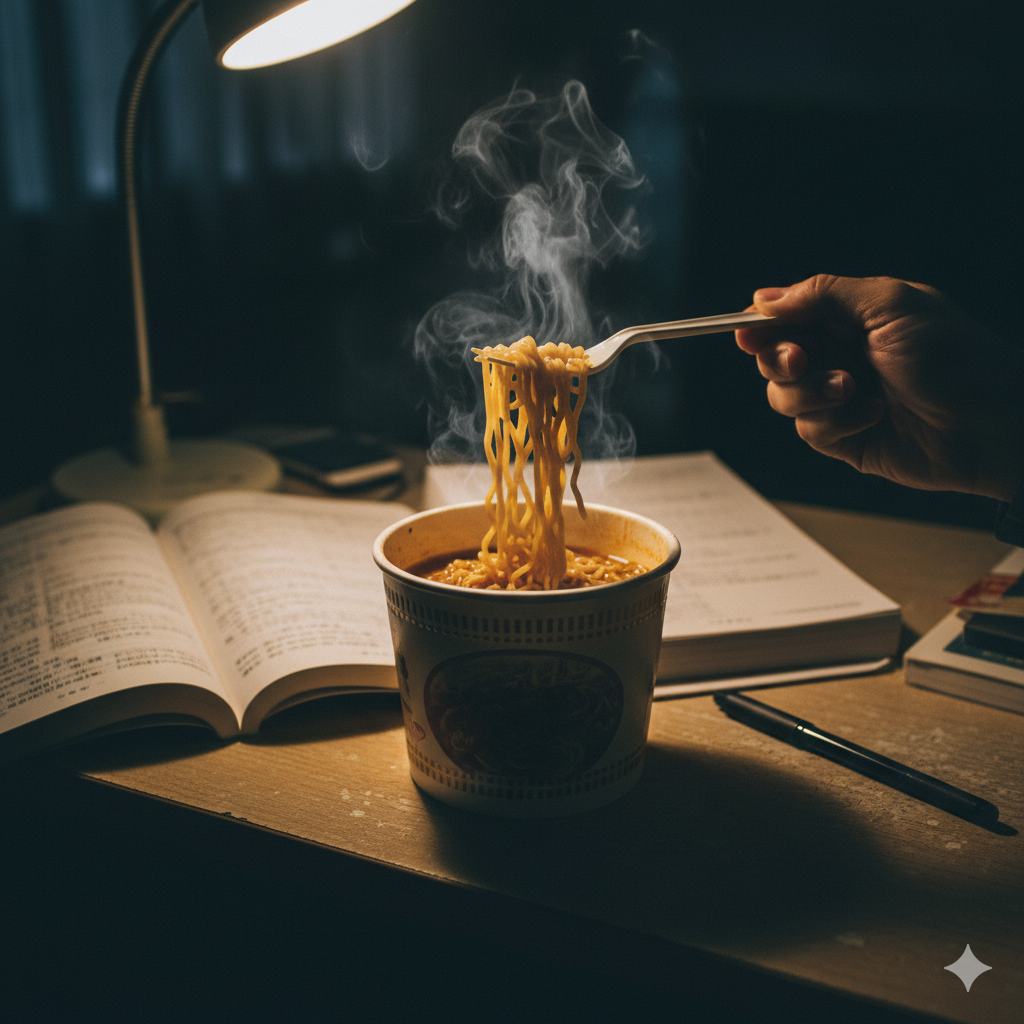
\includegraphics[width=\textwidth]{../images/b0.png}\\[2pt]
  {\footnotesize\color{MidGray} 原图：用户上传}
\end{minipage}
\hfill
\begin{minipage}[t]{0.47\textwidth}
  \centering
  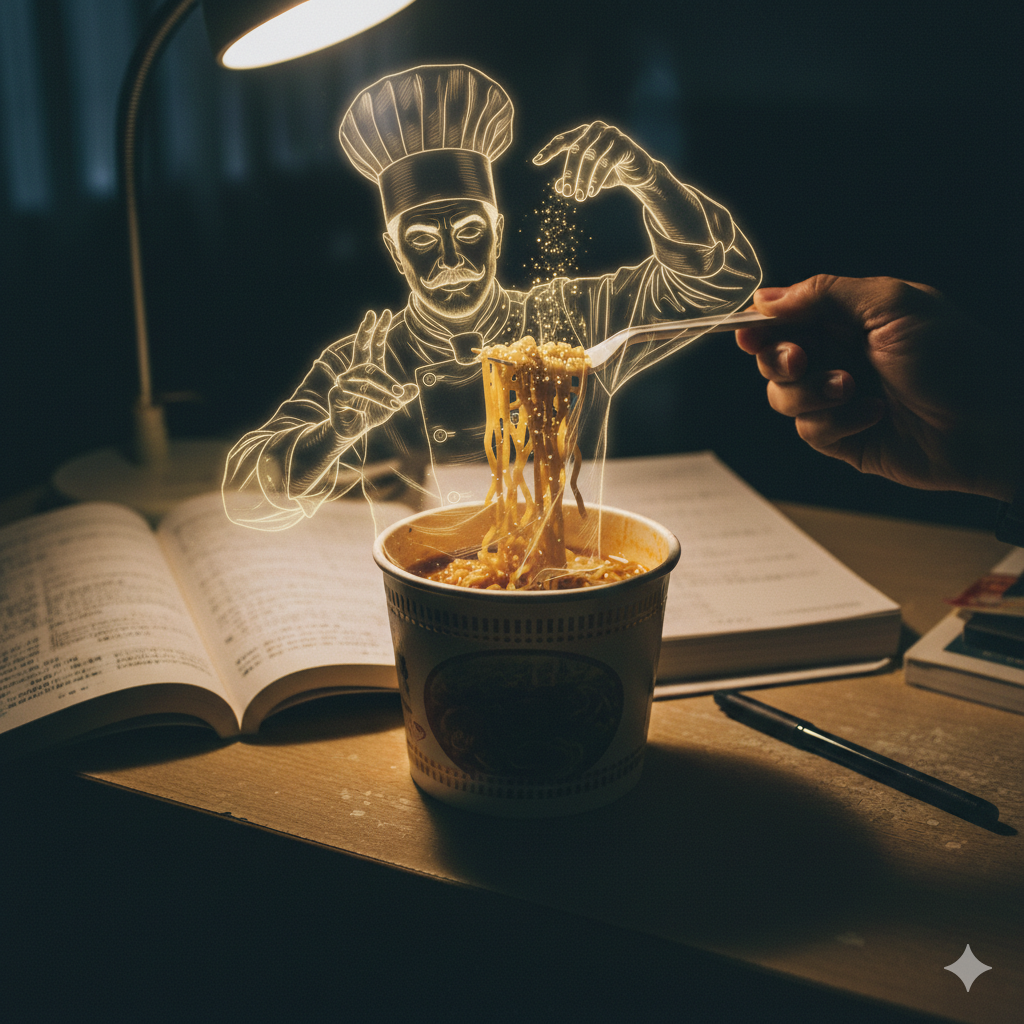
\includegraphics[width=\textwidth]{../images/b1.png}\\[2pt]
  {\footnotesize\color{MidGray} AI 生成结果}
\end{minipage}

%%════════════════════════════════════════════════════════════════
\section{模块二：产品方案设计}
%%════════════════════════════════════════════════════════════════

\subsection{产品概述}

\begin{tcolorbox}[dramabox]
  \kw{一句话定义}：小题大Drama 是一款让年轻人「发一张图，让 AI 把它变得好玩，让 NPC 捧场」的 AI 原生社交产品——把任意日常瞬间（不论倒霉还是幸福），重构成有人懂、有人笑、有人评论的 Drama 现场。
\end{tcolorbox}

\vspace{4pt}
\noindent 产品做三件事：
\begin{enumerate}[leftmargin=2em, itemsep=0.25em, topsep=3pt]
  \item \kw{看懂你的无聊日常}——多模态感知，提取场景实体与情绪标签
  \item \kw{用戏剧化、有反差感的视觉手法重构现实}——在结构约束下，将日常瞬间重绘为有趣、有梗的图片或live图
  \item \kw{一键发布并获得 AI 互动反馈}——5 位 NPC 发布后陆续点赞与评论，消灭社交空窗期
\end{enumerate}

%%── 横向四步 AI 链路概览（TikZ 内联）─────────────────────────
\vspace{6pt}
\begin{center}
\begin{tikzpicture}[node distance = 0.5cm]
  \tikzset{
    pipe/.style = {
      rectangle, rounded corners = 4pt,
      minimum width = 3.4cm, minimum height = 1.0cm,
      align = center, font = \small
    }
  }
  \node[pipe, draw=TokenPurple!70, fill=SoftPurple] (p1)
    {\textbf{感知层}\\{\scriptsize\model{youtu-vita}}};
  \node[pipe, draw=AppleBlue!70,   fill=LightBlue,  right=0.5cm of p1] (p2)
    {\textbf{决策层}\\{\scriptsize\model{hy3-preview}}};
  \node[pipe, draw=AppleBlue!70,   fill=LightBlue,  right=0.5cm of p2] (p3)
    {\textbf{生成层}\\{\scriptsize\model{hy-image / video}}};
  \node[pipe, draw=SupaGreen,      fill=SoftGreen,  right=0.5cm of p3] (p4)
    {\textbf{反馈层}\\{\scriptsize NPC 评论}};
  \draw[->, >=Stealth, line width=1.0pt, color=DarkGray!70]
    (p1.east) -- (p2.west);
  \draw[->, >=Stealth, line width=1.0pt, color=DarkGray!70]
    (p2.east) -- (p3.west);
  \draw[->, >=Stealth, line width=1.0pt, color=DarkGray!70]
    (p3.east) -- (p4.west);
\end{tikzpicture}
\\[3pt]
{\footnotesize\color{MidGray} 产品 AI 全链路概览（感知 $\to$ 决策 $\to$ 生成 $\to$ 反馈）}
\end{center}
\vspace{4pt}

\subsection{核心功能}

\begin{description}[leftmargin=0em, style=nextline, itemsep=0.8em, topsep=3pt]

  \item[\kw{万物皆可 Drama（多模态感知输入）}]\mbox{}\\
    支持上传任意场景图片（JPG / PNG / WebP，$\leq$10\,MB），前端自动等比压缩至适宜尺寸。图片经多模态视觉大模型（\model{youtu-vita}）分析，识别画面中的核心实体、场景状态与情绪标签，输出结构化的感知结果，驱动后续决策层。

  \item[\kw{Guess \& Refine 情绪互动罗盘（决策层）}]\mbox{}\\
    告别冷冰冰的提示词输入框。语言模型（\model{hy3-preview}）根据感知结果自动生成一句共情破冰文案，并同步给出 3 个风格各异的 Drama 改造方向供用户一键选择，完成意图收敛。支持"换一批"，每次重新生成语义不重复的新选项。

  \item[\kw{结构锁定重绘（生成层）}]\mbox{}\\
    原图作为参考图与生成指令一并提交，图像生成模型（\model{hy-image-v3.0}）或视频生成模型（\model{hy-video-1.5}）在物理骨架与空间透视完全锁定的前提下，对材质、光线与氛围进行戏剧化重绘。前端同步展示原图的边缘骨架预览，直观呈现"结构锁定"效果。

  \item[\kw{AI 赛博社交广场（NPC 闭环）}]\mbox{}\\
    用户发布作品后，5 位个性鲜明的 NPC（Emma 冷幽默、Liam 理性克制、Olivia 温柔共情、Noah 真诚直给、Sophia 审美视角）在数秒内陆续点赞与评论，消灭发布后的社交空窗期。用户回复 NPC 评论时，对应角色还会以其人设继续回复，形成真实感互动闭环。

\end{description}

\subsection{产品架构图}

图~\ref{fig:arch} 展示产品的四个 AI 模块接力：用户端负责交互与上传，AI 能力核心完成感知–决策–生成–反馈全链路，技术底座提供模型与数据支撑。

%%──────────────────────────────────────────────────────────────
%% 架构图（TikZ）— 3 列对称布局，节点全中文功能语言
%%──────────────────────────────────────────────────────────────
\begin{figure}[htbp]
\centering
\resizebox{\textwidth}{!}{%
\begin{tikzpicture}[node distance = 0.5cm and 2.2cm]

  %% ── 列 1：用户端（3 节点）────────────────────────────────
  \node[archFE] (u1) {拍照 / 上传日常图片};
  \node[archFE, below=of u1] (u2) {选择 Drama 风格方向};
  \node[archFE, below=of u2] (u3) {社交广场·浏览与互动};

  \begin{scope}[on background layer]
    \node[grpbox={DarkGray},
          fit=(u1)(u2)(u3),
          label={[font=\footnotesize\bfseries,color=DarkGray]above:用户端}]
          (gU) {};
  \end{scope}

  %% ── 列 2：AI 能力核心（4 节点）──────────────────────────
  \node[archAPI, right=2.2cm of u1] (a1) {多模态图像感知\\提取场景·情绪标签};
  \node[archAPI, below=of a1]       (a2) {意图决策与风格路由\\Guess \& Refine 罗盘};
  \node[archAPI, below=of a2]       (a3) {结构锁定内容生成\\图片 / 视频异步重绘};
  \node[archAPI, below=of a3]       (a4) {NPC 社交闭环\\并发点赞·角色评论};

  \begin{scope}[on background layer]
    \node[grpbox={AppleBlue},
          fit=(a1)(a2)(a3)(a4),
          label={[font=\footnotesize\bfseries,color=AppleBlue]above:AI 能力核心}]
          (gA) {};
  \end{scope}

  %% ── 列 3：技术底座（4 节点）─────────────────────────────
  \node[archTH, right=2.2cm of a1] (t1) {视觉理解模型\\youtu-vita};
  \node[archTH, below=of t1]       (t2) {语言与决策模型\\hy3-preview};
  \node[archTH, below=of t2]       (t3) {图像 / 视频生成模型\\hy-image · hy-video};
  %% 留出足够间距，避免 Supabase 组框标签被 TokenHub 组框遮挡
  \node[archSB, below=1.6cm of t3] (t4) {数据库·存储·认证\\Supabase};

  \begin{scope}[on background layer]
    \node[grpbox={TokenPurple},
          fit=(t1)(t2)(t3),
          label={[font=\footnotesize\bfseries,color=TokenPurple]above:腾讯 TokenHub}]
          (gTH) {};
    \node[grpbox={SupaGreen},
          fit=(t4),
          label={[font=\footnotesize\bfseries,color=SupaGreen]above:Supabase}]
          (gSB) {};
  \end{scope}

  %% ── 箭头：用户端 → AI 核心（水平对齐连线）──────────────
  \draw[arr] (u1.east) -- (a1.west);
  \draw[arr] (u2.east) -- (a2.west);
  \draw[arr] (u3.east) -- (a4.west);

  %% ── 箭头：AI 核心 → 技术底座（水平对齐连线）────────────
  \draw[arr] (a1.east) -- (t1.west);
  \draw[arr] (a2.east) -- (t2.west);
  \draw[arr] (a3.east) -- (t3.west);
  \draw[narr] (a4.east) to[out=0,in=180] (t4.west);

\end{tikzpicture}
}%% end resizebox
\caption{小题大Drama 产品架构（用户端 $\to$ AI 能力核心 $\to$ 技术底座）}
\label{fig:arch}
\end{figure}

\subsection{「用户发图 $\to$ AI 回图」逻辑流程图}

图~\ref{fig:flow1} 展示感知–决策–生成核心链路。图~\ref{fig:flow2} 展示生成完成后的发布与 NPC 社交闭环。

%%──────────────────────────────────────────────────────────────
%% 流程图 2a：感知–决策–生成（对称简洁版，[H] 强制就近排版）
%%──────────────────────────────────────────────────────────────
\begin{figure}[H]
\centering
\scalebox{0.88}{%
\begin{tikzpicture}[node distance = 0.6cm and 0.5cm]

  %% ── 开始 / 校验 ─────────────────────────────────────
  \node[term] (start) {用户选择或拖拽图片};
  \node[proc, below=0.7cm of start] (validate)
    {前端格式校验与等比压缩};

  %% 并行分叉坐标
  \coordinate[below=0.5cm of validate] (fk1);

  %% ── 并行 A：左支（上传）──────────────────────────────
  \node[para, below left=0.3cm and 2.0cm of fk1] (forkA)
    {原图上传至云存储\\获取持久化访问地址};

  %% ── 并行 B：右支（感知）──────────────────────────────
  \node[para, below right=0.3cm and 2.0cm of fk1] (forkB)
    {视觉大模型感知图片\\输出场景·情绪结构化理解};

  %% ── 汇合：意图决策 ───────────────────────────────────
  \coordinate[below=2.8cm of fk1] (fk2);
  \node[proc, below=0.4cm of fk2] (guess)
    {意图决策：展示共情破冰文案\\+ 3 个各异的 Drama 改造方向};

  %% ── 主流继续 ─────────────────────────────────────────
  \node[proc, below=of guess]  (select) {用户点击选择一个风格方向};
  \node[proc, below=of select] (submit)
    {提交内容生成任务\\（携带参考图与生成指令）};
  \node[proc, below=of submit] (poll)
    {异步等待生成完成\\（每 3\,s 查询一次进度）};
  \node[term, below=0.6cm of poll] (result)
    {展示生成结果（图片或视频预览）};

  %% ── 箭头 ──────────────────────────────────────────────
  \draw[arr] (start)          -- (validate);
  \draw[arr] (validate.south) -- (fk1);
  \draw[arr] (fk1) to[out=225,in=90] (forkA.north);
  \draw[arr] (fk1) to[out=315,in=90] (forkB.north);
  \draw[arr] (forkA.south) to[out=270,in=180] (guess.west);
  \draw[arr] (forkB.south) to[out=270,in=0]   (guess.east);
  \draw[arr] (guess)  -- (select);
  \draw[arr] (select) -- (submit);
  \draw[arr] (submit) -- (poll);
  \draw[arr] (poll)   -- (result);

\end{tikzpicture}
}%% end scalebox
\caption{感知--决策--生成链路}
\label{fig:flow1}
\end{figure}

生成结果确认后，用户点击「发布到广场」，触发图~\ref{fig:flow2} 所示的发布与 NPC 互动闭环。

%%──────────────────────────────────────────────────────────────
%% 流程图 2b：发布–NPC 社交闭环（[H] 强制就近排版）
%%──────────────────────────────────────────────────────────────
\begin{figure}[H]
\centering
\scalebox{0.88}{%
\begin{tikzpicture}[node distance = 0.55cm and 0.5cm]

  \node[proc] (pub)
    {用户点击「发布到广场」\\（需登录，非演示模式）};
  \node[proc, below=of pub] (createpost)
    {结果图写入云存储\\作品信息持久化至数据库};

  %% NPC 并发两路
  \node[npc, below left=0.7cm and 2.4cm of createpost]  (likes)
    {5 位 NPC 并发点赞\\（直接写入，无需 AI 生成）};
  \node[npc, below right=0.7cm and 2.4cm of createpost] (comments)
    {语言模型为 5 位 NPC\\分别生成个性化角色评论\\（支持多轮回复互动）};

  \node[term, below=2.6cm of createpost] (plaza)
    {跳转作品广场，NPC 点赞与评论\\在 25\,s 内陆续出现};

  %% 箭头
  \draw[arr] (pub) -- (createpost);
  \draw[arr] (createpost.south) to[out=255,in=90] (likes.north);
  \draw[arr] (createpost.south) to[out=285,in=90] (comments.north);
  \draw[arr] (likes.south)    to[out=270,in=180] (plaza.west);
  \draw[arr] (comments.south) to[out=270,in=0]   (plaza.east);

\end{tikzpicture}
}%% end scalebox
\caption{发布--NPC 社交闭环（5 位角色陆续点赞与评论，消灭社交空窗期）}
\label{fig:flow2}
\end{figure}

\subsection{创新与差异化}

相较于美图秀秀滤镜、妙鸭相机或通用 Midjourney：

\begin{description}[leftmargin=0em, style=nextline, itemsep=0.6em, topsep=3pt]
  \item[\kw{免长 Prompt：AI 先共情、用户再选方向}]
    许多通用生图工具以长文本 Prompt 为起点，学习成本较高。小题大Drama 将主路径设计为「看图 $\to$ 一句共情破冰 $\to$ 三个可点的 Drama 方向」，用户以点击完成意图收敛，降低从零写提示词的负担。同类「选项化」或助手式交互在业界亦有出现，本产品的侧重点在于与后续结构约束生图、广场 NPC 反馈形成\textbf{同一产品内}的连贯链路。

  \item[\kw{结构锁定：反差建立在「还认得出原图」之上}]
    写真类产品多强调人像与模板；通用生图工具（含 Midjourney 等）亦支持参考图与多种一致性手段，但对普通用户而言，要在产品化场景里稳定做到「骨架不变、只换氛围与材质」仍需较多经验。小题大Drama 以参考图约束与语义锚定指令为主路径，配合前端对原图边缘的可视化提示，强调\textbf{可感知的结构一致性}，便于「日常图 $\to$ 有梗图」的传播。

  \item[\kw{NPC 闭环：从「出图」延伸到「有人捧场」}]
    常见生图工具多止步于下载或分享链接。小题大Drama 在发布后为 5 位人设各异的 AI 角色触发并发点赞与评论（$\leq$25\,s 内陆续出现），并可延续多轮回复，把情绪反馈纳入同一闭环。市面上亦有 AI 社交、游戏 NPC 等形态；本产品的差异在于将\textbf{多模态感知、选项化决策、参考约束生成与拟真评论}串成面向日常随手拍的一条 Demo 链路，而非单点功能堆叠。
\end{description}

%%════════════════════════════════════════════════════════════════
\section{模块三：AI 原生能力说明}
%%════════════════════════════════════════════════════════════════

\subsection{AI 核心能力}

小题大Drama 深度融合四个 AI 模块，缺任意一环产品链路即断裂：

\vspace{4pt}
\begin{table}[htbp]
  \centering
  \caption{AI 四模块能力矩阵}
  \label{tab:ai}
  \renewcommand{\arraystretch}{1.4}
  %% tmod：表格专用模型名宏，无 \small，确保与第一列基线对齐
  \newcommand{\tmod}[1]{{\ttfamily\color{TokenPurple}#1}}
  \begin{tabularx}{\linewidth}{>{\bfseries}p{1.4cm} p{3.5cm} X}
    \toprule
    层次 & 模型 / 服务 & 职责与实际输出 \\
    \midrule
    \vspace{4pt}感知层
      & \tmod{youtu-vita}\newline（通用 Token Plan / MaaS）
      & 产品的「眼睛」：看懂任意日常图片的主实体、场景环境与情绪底色，输出结构化理解（13 类情绪枚举、6 类图片类型、差异化风格提示）；内置多重容错与情绪校准机制，确保任何图片都能触发有意义的 Drama 改造建议。 \\
    \addlinespace[3pt]
    \vspace{4pt}决策层
      & \tmod{hy3-preview}\newline（HY Token Plan）
      & 产品的「大脑」：输出一句击中情绪的俏皮破冰文案 + 3 个各不相同的 Drama 方向（内嵌结构锚定指令）；同时承担情绪校准、场景描述补全与提示词收敛等辅助推理任务。 \\
    \addlinespace[3pt]
    \vspace{4pt}生成层
      & \tmod{hy-image} / \tmod{hy-video}\newline（通用 Token Plan / MaaS）
      & 产品的「画笔」：在原图参考约束下异步生成图片或短视频；生成结果在发布时永久落盘至云存储，确保广场内容长期可访问，用户不会看到失效的空图。 \\
    \addlinespace[3pt]
    \vspace{4pt}反馈层
      & \tmod{NPC Engine}\newline（hy3-preview）
      & 产品的「嘴巴和捧场团」：为 5 位 NPC 生成差异化角色评论，并支持用户回复后的多轮接话，形成发布后的拟真社交反馈。 \\
    \bottomrule
  \end{tabularx}
\end{table}

\subsection{AI 如何解决痛点（去掉 AI，产品还能成立吗？）}

\begin{tcolorbox}[dramabox]
  \kw{结论：去掉 AI，本产品将彻底崩溃——四个 AI 模块缺一不可，且相互依赖，无法用传统技术等价替代。}
\end{tcolorbox}

\vspace{4pt}
\begin{enumerate}[leftmargin=2em, itemsep=0.35em, topsep=3pt]
  \item \kw{缺乏 AI 视觉理解 → 无法起步}：仅靠规则难以从一张日常照片中稳定推断场景与情绪语境，后续的选项化 Drama 方向也就缺少依据；Guess \& Refine 的前提是机器对图像有可用的语义理解。

  \item \kw{缺乏 AI 可控生成 → 核心价值消失}：传统滤镜多作用于色调与局部；在保留原图透视与主体的前提下做\textbf{语义级}的场景化重绘，依赖生成模型与参考约束，而非普通图像处理滤镜可替代。

  \item \kw{缺乏 LLM 驱动的 NPC → 情绪闭环断裂}：规则机器人只能输出固定回复；只有 LLM 才能针对每张不同的生成图，逐次生成懂梗、拟真、每个角色各具个性的评论，让用户感受到「有人真的看过这张图」。
\end{enumerate}

\subsection{AI 技术方案（感知--决策--生成 任务拆解）}

\subsubsection*{感知层：从图片到结构化语义}

\begin{itemize}[leftmargin=2em, itemsep=0.3em, topsep=3pt]
  \item \kw{开放式视觉理解，任意日常图片均可输入}：\model{youtu-vita} 多模态模型对上传图片做自由文本理解，输出「主实体 + 场景环境 + 情绪氛围 + 风格提示」四维结构，不依赖固定模板匹配——无论用户上传什么，模型都能用自然语言描述画面、判断情绪。

  \item \kw{场景路由：为不同题材微调改造方向}：感知结果包含一个\textbf{场景类型路由标记}，目前按画面主体归为人像、食物、场景、宠物、物品和其他六个方向，对应在系统提示词中给出了不同的 Drama 改造倾向（如食物偏美食插画、宠物偏 Q 版萌化，其他题材则走泛化路线）。此标记服务于\textbf{风格提示的优先级排序}，不限制输入内容——所有题材均可进入完整流程，"其他"类走通用路线仍可产出有意义的改造方向。

  \item \kw{解析兜底，尽量不因格式异常中断链路}：视觉模型返回内容若格式不规范，服务端会依次尝试多种结构映射；若仍不可用，会把原始文本交给混元文本模型按固定 JSON schema 重新整理（两阶段兜底）；情绪置信度偏低时还可触发一次情绪复核。这些机制目的是减少格式漂移带来的链路中断，而非保证 100\% 永不报错。
\end{itemize}

\subsubsection*{决策层：Guess \& Refine——为什么不做 Prompt 输入框}

\begin{itemize}[leftmargin=2em, itemsep=0.3em, topsep=3pt]
  \item \kw{AI 先说话，用户再选择}：系统在展示 3 个选项之前，先输出一句俏皮的破冰点评（如"被 DDL 冲烂了吧哥们？选个姿势发疯："），建立情感共鸣后再引导选择，降低决策心理负担，平均 1 次点击即可完成意图收敛。
  \item \kw{双重因果约束，确保生成不崩}：每个选项的生图指令内嵌四层硬约束——\textbf{尺寸构图锁定}（宽高比与取景范围完全不变）、\textbf{物理骨架锁定}（原图实体身份与位置不变）、\textbf{锚点式 Drama}（新增元素须同时满足「视觉因果」：从图像已有锚点自然生发；以及「情绪因果」：是当前场景情绪的视觉具现，禁止与情绪叙事无关的随机物体插入）、\textbf{真实图层融合}（光源/遮挡/颗粒与原图一致）。评判标准为：观众看到后应说"哦——这说得通"，而非"这是什么鬼"——\textbf{意料之外、情理之中}，不荒诞、不无厘头。
  \item \kw{换一批，真的不重复}：「换一批」功能在规则层和语义层双重保障方向差异化，用户无论点多少次，每批 3 个选项都是全新的改造思路，防止「AI 总在循环」的体验疲倦。
\end{itemize}

\subsubsection*{生成层：风格与结构一致性保障}

风格/场景一致性是赛题的核心难点。小题大Drama 用三层机制彼此咬合解决：

\begin{enumerate}[leftmargin=2em, itemsep=0.3em, topsep=3pt, label=\textbf{\arabic*.}]
  \item \kw{参考图约束（图像层）}：原图作为参考输入直接传递给生图模型，模型在原图物理结构的视觉约束下重绘，而非从零创作——这是保证「原图的现实感」在生成结果中得以保留的根本机制。

  \item \kw{语义锚定指令（文本层）}：每条生图 Prompt 首句强制声明「请严格锁定原图的〔物理元素清单〕，物理骨架完全不变」，在文字层面约束模型不改变实体身份与空间关系，与参考图约束形成双重保障。Drama 元素还须满足「情绪因果」——是场景情绪状态的视觉具现（如焦虑 $\to$ 压迫感倒计时、疲惫 $\to$ 食物蒸汽里的仪式感），禁止与场景情绪叙事无关的随机物体插入，确保生成结果「意料之外、情理之中」。

  \item \kw{边缘骨架可视化（用户感知层）}：前端实时从原图提取结构骨架，在界面上以「结构锁定」徽章形式展示，让用户在等待生成时就能直观感受到「AI 记住了原图的形状」——将技术能力转化为用户可感知的信任感。
\end{enumerate}

\subsubsection*{反馈层：NPC 社交闭环}

\begin{itemize}[leftmargin=2em, itemsep=0.3em, topsep=3pt]
  \item \kw{$\leq$25\,s 内有人捧场}：发布后 5 位 AI 角色在 25 秒内陆续送出点赞和个性化评论，把「社交空窗期」压缩到可忽略的范围。用户感受到的是「这张图有人懂」，而不是刷新无数次的空洞等待。
  \item \kw{5 个真实的「人」，而不是 5 条模板}：Emma 的冷幽默、Liam 的理性克制、Olivia 的温柔共情、Noah 的真诚直给、Sophia 的审美视角——每个角色有稳定人设，针对每张具体的生成图输出专属内容，评论区像真正的朋友在聊天。
  \item \kw{互动可以继续}：用户在广场回复评论后，对应 NPC 会以其角色人设继续回复，实现多轮对话，让发布动作真正打开了一段社交互动，而不是单次的「AI 打赏」。
\end{itemize}

%%════════════════════════════════════════════════════════════════
\section{模块四：加分项}
%%════════════════════════════════════════════════════════════════

\subsection{落地可行性}

\subsubsection*{已落地的工程形态}

本项目已完成从开发到部署的完整闭环，采用全托管 Serverless 架构，无需自建后端服务器。线上地址：\href{https://www.xtddrama.site/}{\texttt{www.xtddrama.site}}。

\vspace{3pt}
\begin{itemize}[leftmargin=2em, itemsep=0.25em, topsep=3pt]
  \item \kw{Vercel}：托管 Next.js\,16 前端与 API Route Handlers；所有含密钥的 AI 调用在 Serverless Function 内完成，密钥不暴露前端 bundle；Edge Cache 加速静态资源。

  \item \kw{Supabase}：Postgres 存储 posts / comments / post\_likes / npc\_profiles 表（已含 RLS 策略，游客可读、写入/删改限本人）；Storage 持久化用户原图与发布结果图；Auth 提供登录与会话管理（基于 \code{@supabase/ssr}，session 存于 cookie）。

  \item \kw{TokenHub}：按当前工程实现拆分为 HY Token Plan（\model{hy3-preview} 文本）与通用 Token Plan / MaaS（\model{youtu-vita}、\model{hy-image-v3.0}、\model{hy-video-1.5}）两套配置；封装层（\code{src/lib/tokenhub.ts}）负责按接口类型选择 Base URL / API Key，并为 MaaS 任务提供 429/5xx 指数退避重试与 30\,s 超时控制。
\end{itemize}

\subsubsection*{稳定性保障措施}

\begin{itemize}[leftmargin=2em, itemsep=0.25em, topsep=3pt]
  \item \kw{演示降级模式}：Vision API 或生图 API 不可用时，自动切换预置 Mock 数据（\code{src/lib/mock-drama-examples.ts}），前端有明确"演示模式"标注；演示模式下禁止发布真实内容，保障 Demo 展示链路完整可用。
  \item \kw{感知两阶段兜底}：\model{youtu-vita} 格式异常时，\model{hy3-preview} 自动二次结构化重组，感知层整体成功率显著提升，避免因模型输出格式漂移导致链路中断。
  \item \kw{镜像落盘}：生成结果 URL 在发布时同步拉取并持久化至 Supabase Storage，广场内容不依赖模型临时 CDN 链接；若拉取失败则拒绝发布并给出明确错误提示。
\end{itemize}

\subsection{商业化思考}

小题大Drama 目前是参赛 Demo，但基础变现逻辑可在 Demo 形态上直接延伸，无需推倒重构：

\vspace{3pt}
\begin{description}[leftmargin=0em, style=nextline, itemsep=0.6em, topsep=3pt]

  \item[\kw{免费 + 会员增值（C 端主线）}]
    基础路径免费（图片生成有次数上限）；视频/Live 图生成、更高分辨率、去水印下载，绑定 QQ 超级会员（SVIP）权益解锁，以腾讯现有会员体系为发行渠道，无需独立支付链路冷启动。

  \item[\kw{情绪 IP 角色（社交付费延伸）}]
    当前 5 位 NPC 为通用角色。后续可引入腾讯在版权影视/游戏/动漫方向已有的 IP（如《王者荣耀》英雄、《甄嬛传》人设），付费解锁专属角色陪玩，在「情绪互动」场景复用 IP 授权价值。此方向与腾讯 PCG 自有内容生态有天然协同。

  \item[\kw{UGC 内容广场的社区运营}]
    广场在 Demo 阶段已具备发布、点赞、评论的基础社区形态。规模化后可引入内容推荐算法，以「今日 Drama 榜」「同城梗图」「话题挑战赛」等运营工具驱动 DAU 增长；创作激励（流量激励/打赏/共创收益分成）可作为创作者留存手段。

  \item[\kw{品牌 \& 营销场景（ToB）}]
    品牌可认购「专属风格库」在特定时间节点向用户曝光（如开学季、游戏新赛季联名风格），用户每次生图即是一次品牌内容的自发传播。算力成本由品牌方承担，平台获得零边际成本的 UGC 裂变。相比传统贴片广告，品牌内容嵌入在「用户主动生成的梗图」中，传播接受度更高。

\end{description}

\subsubsection*{接入腾讯 PCG 业务的可行性}

\vspace{2pt}
小题大Drama 的核心能力（看图 $\to$ 生图 $\to$ 社交反馈）具备较低的接入成本，可作为「AI 视觉互动插件」无缝嵌入 PCG 现有产品：

\vspace{3pt}
\begin{description}[leftmargin=0em, style=nextline, itemsep=0.4em, topsep=2pt]
  \item[\kw{QQ 空间}] 作为"夸张版动态发布"入口，用户发图时增加「小题大作」选项，无需跳出 App；结合空间的社交关系链，NPC 互动可升级为真实好友的优先评论推送。

  \item[\kw{腾讯视频}] 用户截取剧集名场面一键生成 Drama 梗图，以角色人设 NPC 评论互动，打通追剧与二创衍生生态；「剧集专属风格库」可与版权方联动。

  \item[\kw{QQ 群聊 / 频道}] 作为群内轻量 Bot，接收成员发图、生成结果、广播至群内，以「AI 斗图」形式激活群活跃度，降低功能触达门槛。

  \item[\kw{微信（生态延伸）}] 小程序形态可承接微信侧朋友圈分享诉求，用户生成图片一键生成配套「Drama 朋友圈文案」，打通图文一体化分享链路。
\end{description}

%%════════════════════════════════════════════════════════════════
\section*{结语}
\addcontentsline{toc}{section}{结语}
%%════════════════════════════════════════════════════════════════

\begin{center}
「年轻人不缺图，缺的是让一张普通图片值得发出去的那一步——\\[0.35em]
小题大Drama 想做的，就是这一步。」
\end{center}

\noindent 从一张随手拍到有人看、有人评、有人懂，小题大Drama 把感知、决策、生成与反馈串成一条用户可直接感受到的闭环。它是对赛题「AI 玩转视觉互动」的直接作答，也是一次把大模型能力落进年轻人日常表达的实验——从 Demo 起步，向产品化延伸的路径已在。

\end{document}
